\section{Arithmetik}
\subsection{addieren und subtrahieren}
Adieren und Subtrahieren benötigt keine Fallunterscheidung, solange sich die negative Zahl im Zeierkomplement befindet.\\
Es gilt:\\
\begin{table}[h]
\begin{tabular}{ll|l}

MSB & LSB & Resalt \\ \hline
0   & 0   & 0      \\ 
0   & 1   & 1      \\ 
1   & 0   & 1      \\ 
1   & 1   & 0      \\ 
\end{tabular}
\end{table}

Man muss sich bewusst sein, das Resultat von einer Adition liegt im normalen Binärsystem vor. Das Resultat bei einer addition von negativen Zahlen die im Zweierkomplement verrechnet wurde, liegt auch das Resultat im Zweierkommplement vor.

\subsection{Zweierkomplement}
Sobald eine Vorzeichenbelastete Binäre Zahlenvektor zu verarbeiten ist, muss das MSB betrachtet werden.\\
Ist das MSB eine 0 ist der Zahlenvektor postiv. Hat der Zahlenvektor eine 1 als MSB so handelt ich es um einen neagtiven Wert.
\\
Negative binär Werte mussen ins Zweierkomplement gewandelt werden.\\
Vorgenhen:\\
Alle Bits invertieren und beim LSB eine 1 dazu addieren.
\\
Um aus dem Zweierkomplement wider auf einen normalen binären Bitvektor zu gelangen wird das Selbe gemacht\\
Alle Bits invertieren und beim LSB eine 1 dazu addieren.
\begin{figure}[htbp]
	\centering
		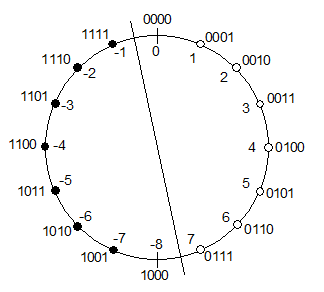
\includegraphics[width=6cm]{content/bilder/Zahlenkreis.png}
	\caption{Vier Bit signed Zahlenkreis Dezimal und Zweierkomplement angebe}%
	\label{Zahlenkreis}
\end{figure}


